%MKB
%Mathematik
%Übungseinheit 3
%Hausübungen
%Aufgabe P7 
\pagebreak
\setcounter{P-section}{7}
\renewcommand*\thesection{P\Nummerierung{\arabic{P-section}}}
\section{Kuboktaeder}

\begin{center}
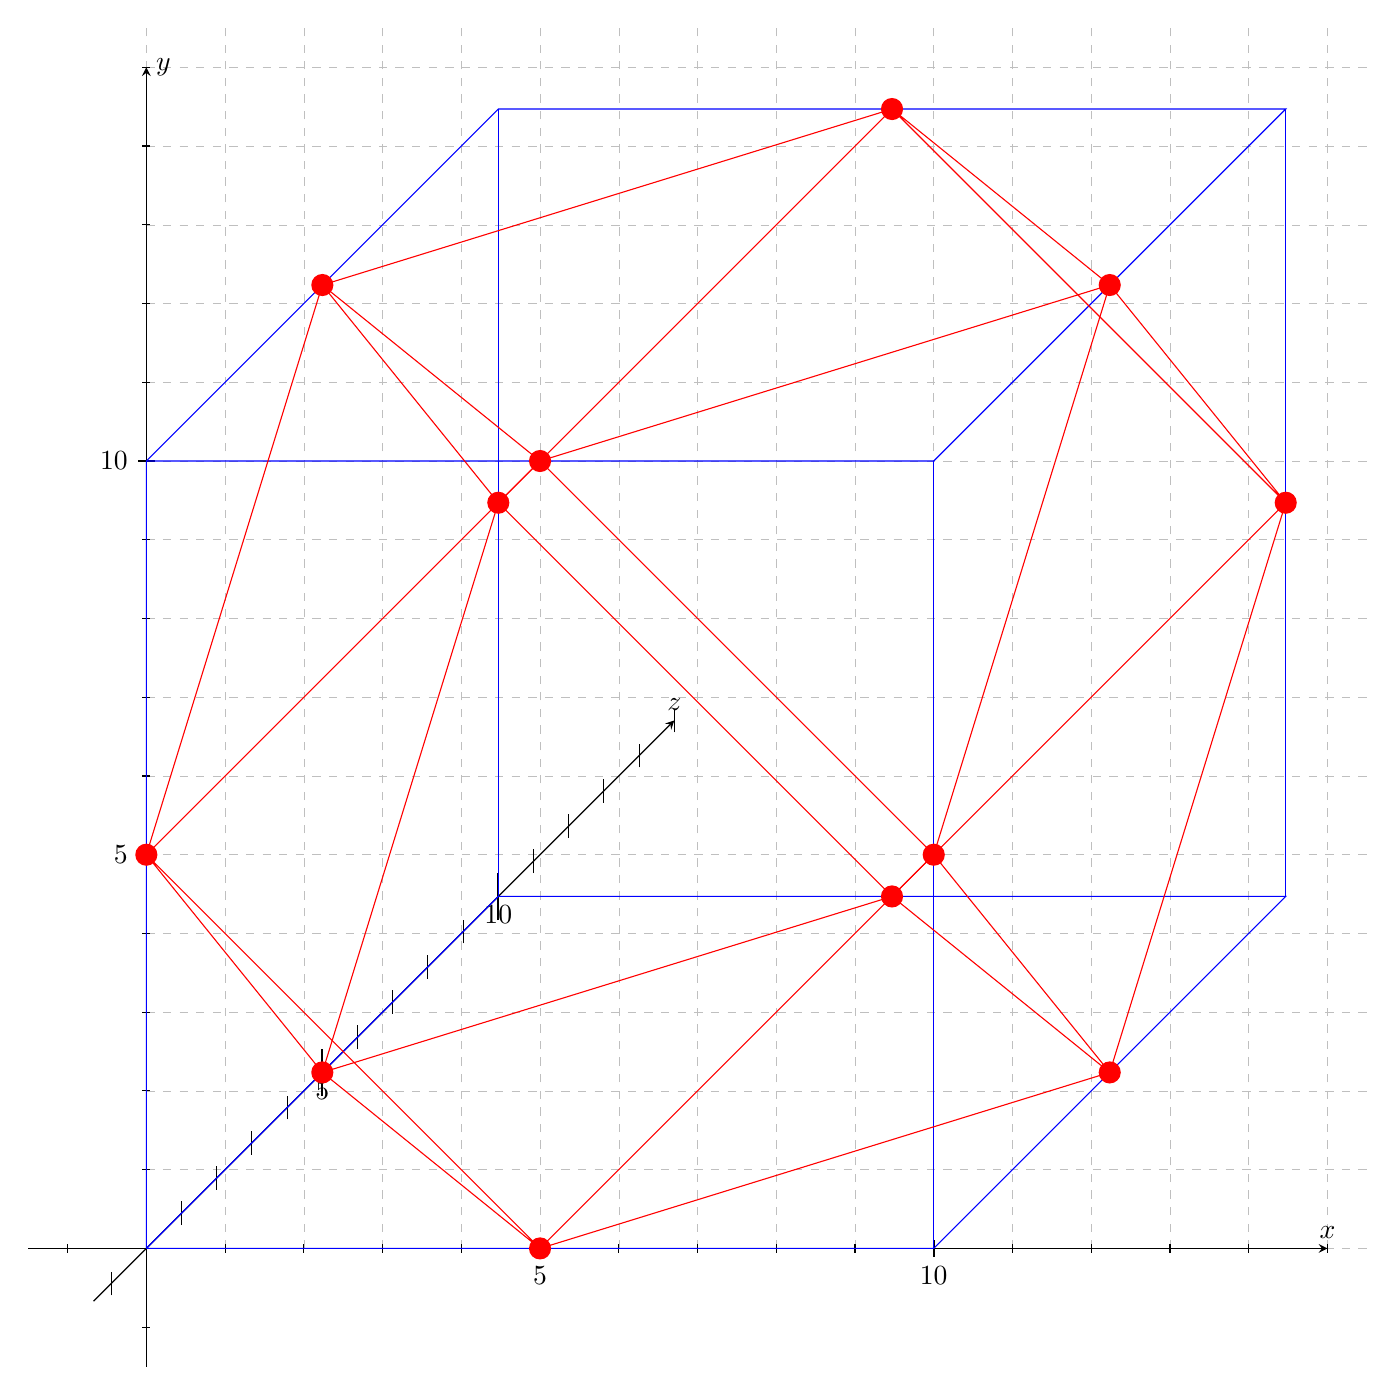
\begin{tikzpicture}[x=1cm,y=1cm,z=0.447cm,>=stealth]
\draw[step=1cm,lightgray,very thin,dashed] (0,15.5) grid (15.5,0);
% The axes
\draw[->] (xyz cs:x=-1.5) -- (xyz cs:x=15) node[above] {$x$};
\draw[->] (xyz cs:y=-1.5) -- (xyz cs:y=15) node[right] {$y$};
\draw[->] (xyz cs:z=-1.5) -- (xyz cs:z=15) node[above] {$z$};
% The thin ticks

\foreach \coo in {-1,0,...,15.5}
{
	\draw (\coo,-1.5pt) -- (\coo,1.5pt);
	\draw (-1.5pt,\coo) -- (1.5pt,\coo);
	\draw (xyz cs:y=-0.15pt,z=\coo) -- (xyz cs:y=0.15pt,z=\coo);
}

% The thick ticks
\foreach \coo in {5,10}
{
	\draw[thick] (\coo,-3pt) -- (\coo,3pt) node[below=6pt] {\coo};
	\draw[thick] (-3pt,\coo) -- (3pt,\coo) node[left=6pt] {\coo};
	\draw[thick] (xyz cs:y=-0.3pt,z=\coo) -- (xyz cs:y=0.3pt,z=\coo) node[below=8pt] {\coo};
}

% Dashed lines for the points P, Q
%\draw[dashed] 
%(xyz cs:z=0) -- +(0,10) -- (xyz cs:y=10) -- +(10,0) -- ++(xyz cs:x=10,z=10) -- +(-10,0) --  ++(xyz cs:x=0,z=0)--+(0,-10);% --cycle;

\draw[blue] (xyz cs:z=0) -- +(0,10)--(xyz cs:y=10)-- +(10,0)--(xyz cs:x=10,y=10,z=10)--+(-10,0)--(xyz cs:x=0,y=10,z=0) ;% --cycle;

\draw[blue] (xyz cs:z=0) -- +(10,0)-- (xyz cs:x=10,z=10)--+(-10,0)--(xyz cs:x=0,z=0);

\draw[blue] (xyz cs:x=10,y=0,z=0) -- (xyz cs:x=10,y=10,z=0);
\draw[blue] (xyz cs:x=10,y=0,z=10) -- (xyz cs:x=10,y=10,z=10);
\draw[blue] (xyz cs:x=0,y=0,z=10) -- (xyz cs:x=0,y=10,z=10);

%Above 
\draw[red] (xyz cs:x=0,y=5,z=0) -- (xyz cs:x=5,y=10,z=0)--(xyz cs:x=0,y=10,z=5)--(xyz cs:x=0,y=5,z=0);
\draw[red] (xyz cs:x=0,y=10,z=5) -- (xyz cs:x=0,y=5,z=10)--(xyz cs:x=5,y=10,z=10)--(xyz cs:x=0,y=10,z=5);
\draw[red] (xyz cs:x=5,y=10,z=10) -- (xyz cs:x=10,y=5,z=10)--(xyz cs:x=10,y=10,z=5)--(xyz cs:x=5,y=10,z=10);
\draw[red] (xyz cs:x=10,y=10,z=5) -- (xyz cs:x=10,y=5,z=0)--(xyz cs:x=5,y=10,z=0)--(xyz cs:x=10,y=10,z=5);

%Bottom
\draw[red] (xyz cs:x=0,y=5,z=0) -- (xyz cs:x=0,y=0,z=5)--(xyz cs:x=5,y=0,z=0)--(xyz cs:x=0,y=5,z=0);
\draw[red] (xyz cs:x=0,y=0,z=5) -- (xyz cs:x=0,y=5,z=10)--(xyz cs:x=5,y=0,z=10)--(xyz cs:x=0,y=0,z=5);
\draw[red] (xyz cs:x=5,y=0,z=10) -- (xyz cs:x=10,y=5,z=10)--(xyz cs:x=10,y=0,z=5)--(xyz cs:x=5,y=0,z=10);
\draw[red] (xyz cs:x=5,y=0,z=0) -- (xyz cs:x=10,y=5,z=0)--(xyz cs:x=10,y=0,z=5)--(xyz cs:x=5,y=0,z=0);

\fill[red] (xyz cs:x=0,y=5,z=0) circle (4pt);
\fill[red] (xyz cs:x=5,y=10,z=0) circle (4pt);
\fill[red] (xyz cs:x=0,y=10,z=5) circle (4pt);
\fill[red] (xyz cs:x=0,y=5,z=10) circle (4pt);
\fill[red] (xyz cs:x=5,y=10,z=10) circle (4pt);
\fill[red] (xyz cs:x=10,y=10,z=5) circle (4pt);
\fill[red] (xyz cs:x=10,y=5,z=10) circle (4pt);
\fill[red] (xyz cs:x=10,y=5,z=0) circle (4pt);
\fill[red] (xyz cs:x=10,y=0,z=5) circle (4pt);
\fill[red] (xyz cs:x=5,y=0,z=10) circle (4pt);
\fill[red] (xyz cs:x=0,y=0,z=5) circle (4pt);
\fill[red] (xyz cs:x=5,y=0,z=0) circle (4pt);

\end{tikzpicture}
\end{center}
\textbf{Kuboktaeder:} \\
\\
Ecken($e$): 12\\
\\
Kanten($k$): 24\\
\\
Fl"achen:($f$): 14\\
\\
Die eulersche Polyederformel lautet: e - k + f = 2. Wenn man die Werte f"ur die Ecken, Kanten und Fl"achen des Kuboktaeder einsetzt bekommt man: 12 - 24 + 14 = 2. Daraus erschlie"st sich, dass die eulersche Polyederformel erf"ullt ist.